The current generator is audited on 2,048 consecutive layout seeds (24000--26047) at furnishing density 0.65, static human density 0.25, four cameras and default baseline $b=0.5$. All layouts pass geometry, swept collision and sampled camera constraints. The population contains 508 numeric series, 406 with nonzero observed variance. These are correlated measurements.

The rendered population contains 512 distinct consecutive rooms (24000--24511), four $320\times240$ cameras and times $0,0.5,1$. The first 128 rooms are additionally captured at $b=0,0.25,0.75,1$, yielding 1,024 room/configuration captures and 12,288 views. Every row in the parameter sweep uses the same 128 rooms, with identical geometry, people, materials and lighting, verified by manifest hashes. No failed, dark, or low-overlap sample is replaced. Native Auto lighting and shadows are enabled; baked diffuse GI is disabled for the sweep. The selected gallery uses a separate full-lighting recipe. Captures use the checkout-local wgpu command-cache/upload optimizations; published crates resolve registry wgpu. Timing observations do not qualify unpatched package performance.

\begin{table}[ht]\centering\small
\begin{tabular}{rrrrrr}\toprule
Baseline & Distance (m) & Overlap (\%) & Shared (\%) & All three (\%) & Proxy misses\\\midrule
0.00 & 0.19 & 72.8 & 92.1 & 61.0 & 177 / 1152 \\
0.25 & 1.33 & 55.2 & 85.2 & 39.9 & 96 / 1152 \\
0.50 & 2.19 & 46.5 & 80.7 & 28.4 & 52 / 1152 \\
0.75 & 2.94 & 38.9 & 76.9 & 22.0 & 22 / 1152 \\
1.00 & 3.60 & 32.9 & 72.8 & 17.3 & 11 / 1152 \\
\bottomrule\end{tabular}
\caption{Absolute measurements at five settings of the current camera program. Distance is the median room-mean reference distance, measured at 33 times. Overlap averages bidirectional reference pairs at three rendered times. Shared and all-three fractions use valid source-pixel observations. Each row contains 128 rooms, 1,536 views and 1,152 reference pairs; its proxy threshold depends on baseline.}
\end{table}
\begin{figure}[ht]\centering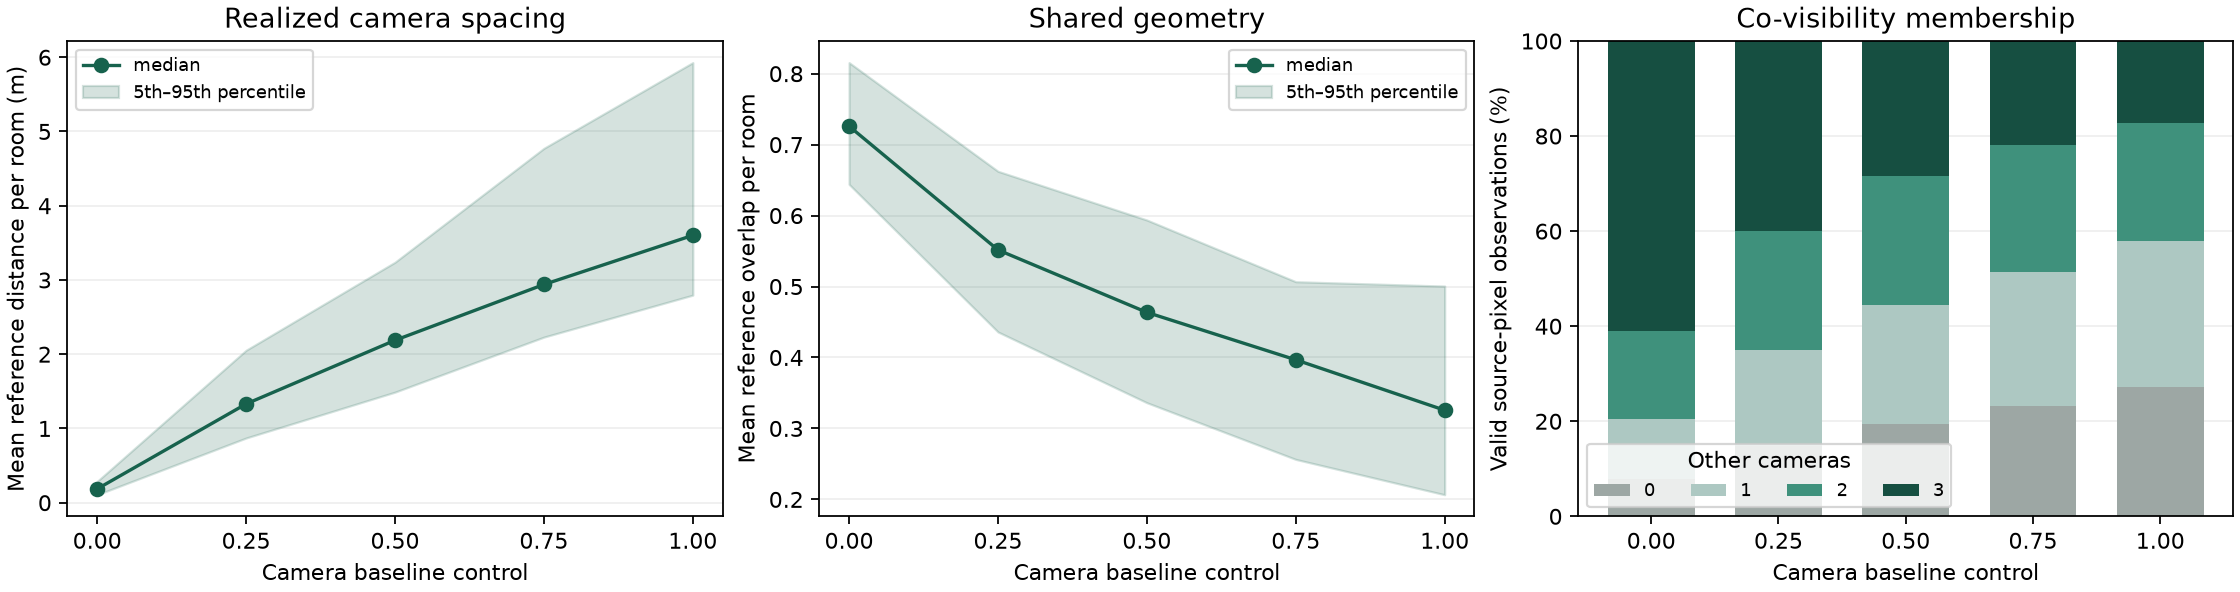
\includegraphics[width=\linewidth]{generated/baseline_sweep.png}
\caption{Realized spacing, room-level overlap quantiles and co-visibility cardinality versus the camera-baseline parameter. Pixel observations and views from the same room are correlated.}\end{figure}
\begin{figure}[ht]\centering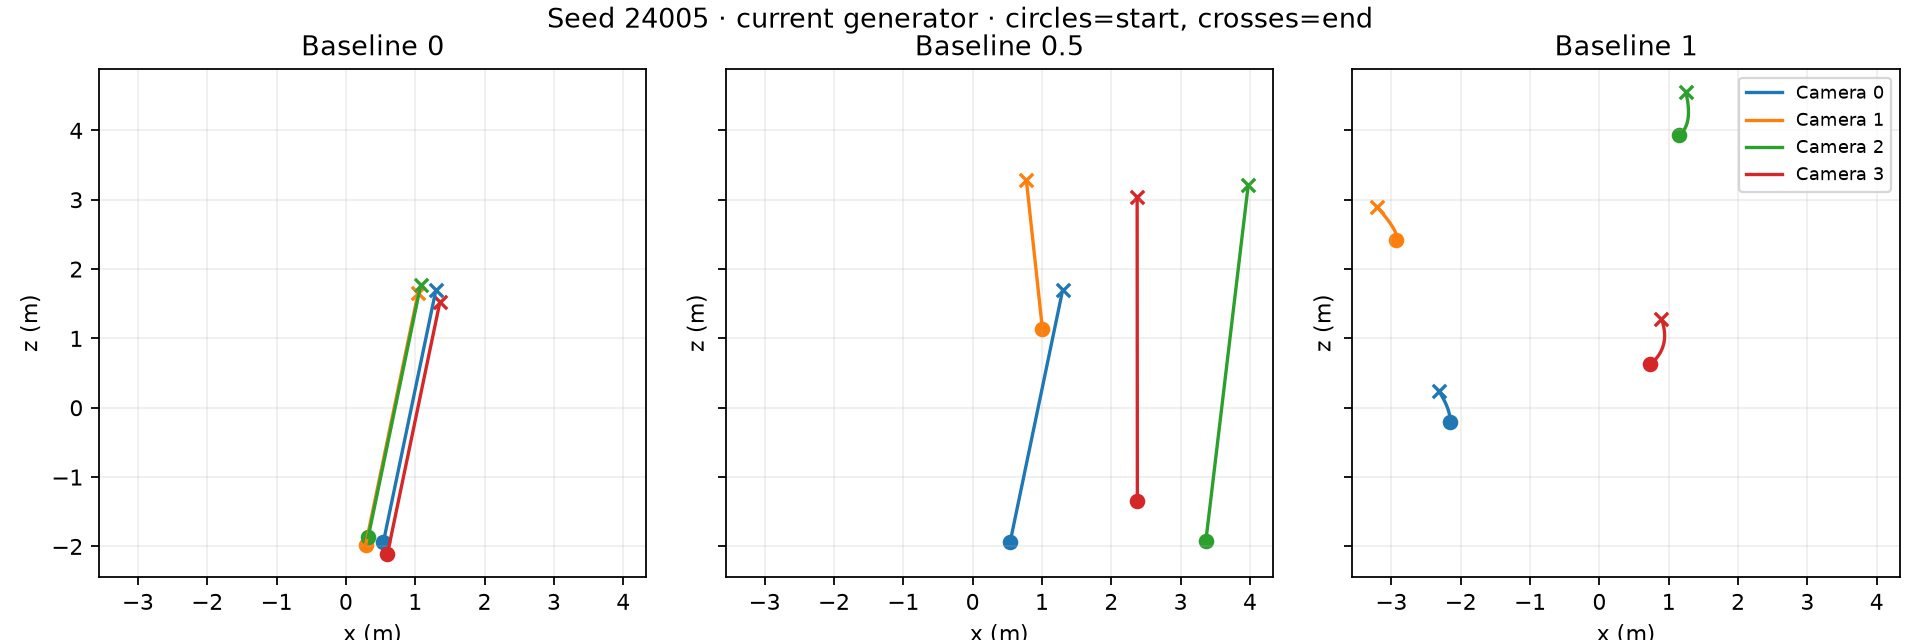
\includegraphics[width=\linewidth]{generated/baseline_paths.png}
\caption{Current camera programs for one fixed room at three baseline settings, using common metric axes.}\end{figure}

At default baseline, all 512 rooms contribute 6,144 views and 4,608 reference-pair/time observations. Mean reference overlap is 45.7\%, with minimum 16.0\%; 210 pairs miss the proxy target. 80.3\% of valid source-pixel observations are visible to another camera, and 27.9\% to all three others. The denominator is 471,859,200 valid pixel observations, not unique 3D points. Membership excludes the source camera.

The independent diagnostic requires nearest-target-pixel depth agreement within $0.01\,\mathrm{m}+0.002z$. The production GPU annotation uses a separate symmetric tangent-plane predicate; its exact masks are exported with the gallery. Both use the first geometric surface, treating glass as annotation-opaque. Reflections and refractions are not counted as geometric correspondence.

There are 0 rooms with a view containing at most two semantic classes, and 0 of 357 occupied primary rooms have no person pixels in any captured view. Maximum per-view p99 depth/position disagreement is 0.0000038\,m. These are annotation and coverage checks, not photographic-realism metrics. Complete distributions, source identities, configurations and commands are in \texttt{docs/camera\_baseline\_v21.md}. Bounded capture processes do not establish unlimited-process memory stability.
